\documentclass[12pt, oneside]{report}

\usepackage[left=2.5cm, top=2.5cm, bottom=2.5cm, right=2.5cm]{geometry}

\usepackage[utf8]{inputenc}
\usepackage[T1]{polski}
\usepackage[polish]{babel}
\usepackage{hyperref}
\usepackage{physics}
\usepackage{graphicx}
\usepackage{amsthm}

\newtheorem{theorem}{Theorem}
\newtheorem{lemma}{Lemma}
\newcommand\Omicron{O}

\begin{document}  
\thispagestyle{empty}
\begin{titlepage}
    \begin{center}

           \Large
    \textbf{Uniwersytet Jagielloński w Krakowie}\vspace{0.2cm}\\ Wydział Matematyki i Informatyki
               \vspace*{1cm}
               
         \vspace{3cm}
         \Large
          \textbf{Pola Kyzioł}\\\vspace{0.5cm}
         \normalsize Nr albumu: 1092406\\
             \vspace{2cm}
        \Huge
        \textbf{Tytuł pracy dyplomowej}
      
        \vspace{1.5cm}
        \normalsize
        Praca magisterska\\
        na kierunku Informatyka Analityczna\\ \vspace{0.15cm}
        
        \vfill
        \vspace{2cm}
       \begin{minipage}{1\textwidth}
\begin{flushright}
Praca wykonana pod kierunkiem\\
dr hab. Tomasz Krawczyk\\
Instytut Informatyki Analitycznej 
\end{flushright}
\end{minipage}
        
        \vspace{2cm}
        \begin{center}
      Kraków 2019
        \end{center}
    \end{center}
\end{titlepage}

\newpage 
 \thispagestyle{empty}
\vspace{2.5cm}
\begin{flushleft}
\large \textbf{Oświadczenie autora pracy}\vspace{0.6cm}\\
\end{flushleft}

\noindent Świadom odpowiedzialności prawnej oświadczam, że niniejsza praca dyplomowa została napisana przeze mnie samodzielnie i nie zawiera treści uzyskanych w sposób niezgodny z obowiązującymi przepisami.\\

\noindent Oświadczam również, że przedstawiona praca nie była wcześniej przedmiotem procedur związanych z uzyskaniem tytułu zawodowego w wyższej uczelni.
\vspace{2cm}
\begin{center}
\begin{tabular}{lr}
................................~~~~~~~~~~~~~~~~~~~~~~~~~~~~~~~~~~~~~~&
.......................................... \\
{~~~~Kraków, dnia} & {Podpis autora pracy~~~~}
\end{tabular}
\end{center}
\vspace{5cm}
\begin{flushleft}
\large \textbf{Oświadczenie kierującego pracą}
\end{flushleft}

\noindent Potwierdzam, że niniejsza praca została przygotowana pod moim kierunkiem i~kwalifikuje się do przedstawienia jej w postępowaniu o nadanie tytułu zawodowego.
\vspace{2cm}
\begin{center}
\begin{tabular}{lr}
................................~~~~~~~~~~~~~~~~~~~~~~~~~~~~~~~~~~~~~~&
............................................ \\
{~~~~Kraków, dnia} & {Podpis kierującego pracą~~}
\end{tabular}
\end{center}
\vfill

\newpage
\tableofcontents

\newpage
  	\chapter{Dekompozycja drzewowa}
  		\section{Definicja dekompozycji i szerokości drzewowej}

Dekompozycją drzewową grafu $G$ nazywamy parę $\mathcal{T} = (T, \{X_t : t \in V(T)\})$, gdzie $T$ jest drzewem, a $\{X_t : t \in V(T)\}$
zawiera zbiory wierzchołków grafu $G$ i spełnia następujące warunki:
\begin{itemize}
	\item{Dla każdej krawędzi $\{u, v\} \in E(G)$, istnieje węzeł $t \in V(T)$, taki że $u \in X_t$ i $v \in X_t$.}
	\item{Dla każdego wierzchołka $v \in V(G)$, zbiór $\{t \in V(T): v \in X_t \}$ jest poddrzewem drzewa $T$.}
\end{itemize}
Od tej pory wierzchołki grafu wyjściowego $G$ będą nazywane po prostu \emph{wierzchołkami}, natomiast węzły drzewa $T$ będą nazywane \emph{kubełkami}.
\newline\newline
Szerokość drzewowa dekompozycji drzewowej $\mathcal{T}$ jest zdefiniowana następująco: \newline $sd_\mathcal{T} = max_{t \in V(T)} \abs{X_t - 1}$. Natomiast szerokość drzewowa grafu $G$ jest minimalną szerokością drzewową wziętą po wszystkich możliwych dekompozycjach drzewowych $G$: \newline $sd_G = min \{sd_\mathcal{T}: \mathcal{T} \text{ jest dekompozycją drzewową }G\}$.
  		
  		\section{Ładna dekompozycja drzewowa}
Dla uproszczenia posługiwania się dekompozycją drzewową przy definiowaniu algorytmów dynamicznych, będziemy używać tzw. \emph{ładnej dekompozycji drzewowej}, która została po raz pierwszy wprowadzona przez Kloks \cite{kloks}.
\newline\newline
\emph{Ładna dekompozycja drzewowa} $\mathcal{T} = (T, \{X_t\}_{t \in V(T)})$ musi spełniać następujące warunki:
\begin{itemize}
	\item{$T$ jest ukorzenione.}
	\item{Każdy \emph{kubełek} $T$ ma co najwyżej dwoje dzieci.}
	\item{Jeśli \emph{kubełek} $t$ ma dwoje dzieci $p$ i $q$, wtedy $X_t = X_p = X_q$.}
	\item{Jeśli \emph{kubełek} $t$ ma jedno dziecko $p$, to $\abs{X_t} = \abs{X_p} + 1$ \emph{oraz} $X_p \subset X_t$ albo $\abs{X_t} = \abs{X_p} - 1$ \emph{oraz} $X_t \subset X_p$.}
\end{itemize}
Ponieważ w ładnej dekompozycji drzewowej, \emph{kubełki} różnią się od siebie o co najwyżej jeden \emph{wierzchołek}, każde przejście między jednym a drugim \emph{kubełkiem} odpowiada dokładnie jednej operacji na grafie wyjściowym $G$. Każdy \emph{kubełek} ma jeden z następujących pięciu typów:
\begin{itemize}
	\item{\texttt{WPROWADZAJĄCY v} - \emph{kubełek} ten ma o jeden \emph{wierzchołek} więcej niż jego jedyne dziecko: $X_p \cup \{v\} = X_t$. Każdy wierzchołek $v \in V(G)$, ma co najmniej jeden kubełek wprowadzający.}
	\item{\texttt{ZAPOMINAJĄCY v} - \emph{kubełek} o jednym wierzchołku mniej niż jedgo jedyne dziecko: $X_t \cup \{v\} = X_p$. Jego specjalnym reprezentantem jest korzeń. Dla każdego wierzchołka $v \in V(G)$, istnieje dokładnie jeden kubełek zapominający.}
	\item{\texttt{SCALAJĄCY} - jedyny \emph{kubełek} posiadający dwoje dzieci: $X_t = X_p = X_q$, scala dwa podgrafy o przecięciu $X_t$.}
	\item{\texttt{LIŚĆ} - dla $t$ będącego liściem: $X_t = \emptyset$.}
	\item{\texttt{UZUPEŁNIAJĄCY uv} - \emph{kubełek}, który nie pojawił się w pierwotnej definicji ładnej dekompozycji drzewowej, ale ułatwia definiowanie algorytmów operujących na dekompozycjach drzewowych. \emph{Kubełek} uzupełniający wprowadza krawędź $uv \in E(G)$ (uzupełnia krawędziami reprezentację grafu $G$ w drzewie $T$). \emph{Kubełek} $t$ \texttt{UZUPEŁNIAJĄCY} $uv$ zawiera oba \emph{wierzchołki} krawędzi: $u \in X_t$ i $v \in X_t$. Dla każdego $uv$ istnieje dokładnie jeden kubełek uzupełniający i - przyjmując bez straty ogólności $t(u)$ jest przodkiem $t(v)$ (gdzie $t(v)$ to najwyższy \emph{kubełek}, taki że $v \in X_{t(v)}$) - znajduje się on pomiędzy $t(v)$ a \texttt{ZAPOMINAJĄCY v}.}
\end{itemize}

daj tu przykład
		\section{Obliczanie dekompozycji drzewowej}

Problem obliczania dekompozycji drzewowej należy do klasy problemów FPT. Odkąd Robertson i Seymour \cite{robertson&seymour} wprowadzili w latach osiemndziesiątych definicję dekompozycji drzewowej i jako pierwsi podali parametryzowany algorytm znajdowania dekompozycji drzewowej rozmiaru $\Omicron(k)$ (dla pewnej stałej $k$) o czasie działania $\Omicron(n^{f(k)})$ na grafie $n$-wierzchołkowym ($f(k)$ nigdy nie obliczyli), zostało opublikowanych wiele nowych, wielomianowych algorytmów parametryzowanych o znacznie lepszych złożonościach czasowych. Jednakże Bodlaender \cite{bodlaender} jako pierwszy podał liniowy algorytm znajdowania dekompozycji drzewowej o szerokości $k$ (o ile taka dekompozycja istnieje). 

\begin{theorem}[Bodlaender]
Dla wszystkich $k \in N$ istnieje algorytm działający w czasie liniowym, który dla danego grafu $G = (V, E)$ sprawdza, czy szerokość drzewowa tego grafu wynosi co najwyżej $k$ oraz - jeśli tak - oblicza dekompozycję drzewową $G$ o szerokości drzewowej co najwyżej $k$.  
\end{theorem}

Ponadto Kloks \cite{kloks} pokazał, że dla każdego grafu o szerokości drzewowej $k$ istnieje ładna dekompozycja drzewowa, którą można skonstruować w czasie liniowym od ilości wierzchołków grafu wyjściowego $G$.

\begin{lemma}[Kloks]
\label{kloks}
Każdy graf $G$ o szerokości drzewowej $k$ posiada ładną dekompozycję drzewową o szerokości $k$. Ponadto, jeśli $G$ jest grafem $n$-wierzchołkowym, to istnieje ładna dekompozycja drzewowa grafu $G$ o co najwyżej $4n$ kubełkach.
\end{lemma}

\begin{proof}[Dowód indukcyjny]
Graf $G$ ma szerokość drzewową $k$, wobec czego ma co najmniej $k+1$ wierzchołki. Ponadto każdy graf o szerokości drzewowej $k$ da się striangulować do postaci $k$-drzewa. Triangulacja grafu $G$ do $k$-drzewa opiera się na znalezieniu zrównoważonej dekompozycji drzewowej $\mathcal{T} = (T, \{X_t\}_{t \in V(T)})$, w której dla każdego $t \in V(T)$: $\abs{X_t} = k+1$ oraz dla każdej krawędzi $(t, p) \in E(T)$: $\abs{X_t \cap X_p} = k$, a następnie na dodaniu do $G$ krawędzi między każdą parą wierzchołków $(u, v)$, dla której istnieje kubełek nowo powstałej dekompozycji $t$ : $u \in X_t$ $\wedge$ $v \in X_t$. Algorytm równoważenia dekompozycji drzewowej został przedstawiony przez Bodlaender \cite{bodlaender} i działa on w czasie liniowym. Niech $H$ będzie striangulowanym grafem $G$ o $n$ wierzchołkach. Indukcyjnie można pokazać, że istnieje ładna dekompozycja grafu $H$ o szerokości drzewowej $k$ (w tym twierdzeniu ładna dekompozycja nie zakłada, że liście są puste).
\begin{description}
\item[Dla $n=k+1$,]{możemy wziąć trywialną dekompozycję drzewową, tj. umieścić wszystkie wierzchołki w jednym kubełku.}
\item[Dla $n>k+1$,]{$H$ posiada wierzchołek $v$, którego sąsiedzi tworzą klikę. Niech $H^{\prime}$ będzie grafem otrzymanym z $H$ poprzez usunięcie wierzchołka $v$. Z indukcji dostajemy, że istanieje ładna dekompozycja drzewowa $H^{\prime}$ o co najwyżej $4(n-1)$ kubełkach. Niech $S$ oznacza zbiór sąsiadów wierzchołka $v$. Ponieważ $S$ jest kliką (rozmiaru $k$), musi istnieć kubełek $X_t$ ładnej dekompozycji drzewowej, który zawiera $S$. Rozważmy trzy następujące przypadki dotyczące kubełka $t$:
\begin{enumerate}
\item{$t$ ma dwoje dzieci $p$ i $q$, wobec czego $X_t = X_p = X_q$. Schodzimy w dół drzewa do dowolnego z dzieci i kontynuujemy aż nie znajdziemy się w kubełku $p$ o co najwyżej jednym dziecku.}
\item{$p$ jest liściem. Jeśli $X_p = S$, tworzymy nowy kubełek $a$: $X_a = S \cup \{v\}$, który staje się dzieckiem $p$. Wpp. $X_p \neq S$, niech $z \in X_p \setminus{S}$, $p$ dostaje nowe dziecko $a$: $X_a = X_p \setminus \{z\}$. Ponieważ $S \subset X_p$ i $k = \abs{S} \leq k+1$, $X_a = S$. Dodajemy kolejny kubełek $b$ jako dziecko $a$: $X_b = S \cup {v}$.}
\label{przypadek2}
\item{$p$ ma jedno dziecko $q$. Usuwamy krawędź $(p, q)$ z drzewa. Tworzymy nowy kubełek $a$: $X_a = X_p$ i dodajemy go do drzewa jako dziecko $p$, natomiast $q$ podpinamy jako dziecko $a$. Tworzymy kolejny nowy kubełek $b$: $X_b = X_p$ i podpinamy $b$ jako dziecko $p$ (drugie dziecko). Schodzimy w dół drzewa do kubełka $b$, który jest liściem i postępujemy zgodnie z \ref{przypadek2}. Łatwo zauważyć, że wprowadzimy co najwyżej 4 nowe wierzchołki.} 
\end{enumerate}
Ponieważ dekompozycja drzewowa dla $H^{\prime}$ ma co najwyżej $4(n-1)$ wierzchołki, dekompozycja drzewowa dla $H$ ma co najwyżej $4n$ wierzchołki, co kończy dowód.}
\end{description}
\end{proof}

\begin{lemma}[Kloks]
Dla stałej $k$, mając daną dekompozycję drzewową grafu $G$ o szerokości $k$ i $\Omicron(n)$ wierzchołkach, gdzie $n$ jest liczbą wierzchołków grafu $G$, da się skonstruować ładną dekompozycję drzewową grafu $G$ o szerokości $k$ i co najwyżej $4n$ kubełkach w czasie $\Omicron(n)$. 
\end{lemma}

\begin{proof}
Dowód opiera się na konstrukcji przedstawionej w dowodzie lematu \ref{kloks}. Konstrukcja ta wymaga na wejściu striangulowanego grafu $G$ do postaci $k$-drzewa, triangulacja wymaga czasu liniowego. Szukanie odpowiedniej kolejności usuwania kubełków z $k$-drzewa $H$, czyli takiej w której sąsiedzi usuwanego kubełka indukują klikę, jest również liniowe. Dowód lematu wynika już teraz bezpośrednio z konstrukcji przedstawionej w dowodzie lematu \ref{kloks}.
\end{proof}

\newpage
  	\chapter{Klasyczne algorytmy dynamiczne}
    	\section{Drzewo Steinera}

Niniejszy algorytm został przedstawiony przez ... Mamy dany nieskierowany graf $G$ oraz zbiór wierzchołków $K$ będący podzbiorem $V(G)$, $K \subset V(G)$. Wierzchołki te nazywane są terminalami.
Naszym zadaniem jest znalezienie dla grafu $G$ takiego jego spójnego podgrafu $H$, który zawiera wszystkie terminale i jego rozmiar jest minimalny.
Zakładamy, że mamy daną ładną dekompozycję drzewową grafu wyjściowego $G$ : $\mathcal{T} = (T, \{X_t\}_{t \in V(T)})$. Dodatkowo, dla uproszczenia samego algorytmu, przyjmujemy, że każdy \emph{kubełek} zawiera przynajmniej jeden terminal. Możemy to łatwo osiągnąć - wybieramy dowolny wierzchołek ${v*}$ będący terminalem (terminale będą dla ułatwienia dodatkowo oznaczane przez *) i dodajemy go do każdego kubełka, usuwamy $\texttt{WPROWADZAJĄCY v}$ i $\texttt{ZAPOMINAJĄCY v}$, własność ładnej dekompozycji drzewowej jest zachowana z tą małą modyfikacją, że liście i korzeń nie są puste.
\newline
Zanim przejdziemy do zdefiniowania algorytmu dynamicznego dla problemu Steinera, wprowadźmy kilka dodatkowych oznaczeń.
Dla kubełka $t$, definiujemy:
\begin{description}
\item[$V_t:$]{suma wszystkich kubełków w poddrzewie ukorzenionym w $t$, włączając $X_t$, inaczej mówiąc wszystkie wierzchołki grafu wyjściowego $G$, które pojawiły się w danym poddrzewie}
\item[$E_t:$]{wszystkie krawędzie $(u, v)$, które zostały zrealizowane w poddrzewie ukorzenionym w $t$, czyli dla których istnieje kubełek $p$: $u \in X_p$ $\wedge$ $v \in X_p$} 
\item[$G_t = $]{$(V_t, E_t)$}
\end{description}

Niech $H$ będzie szukanym drzewem Steinera łączącym wszystkie terminale $K$, a $t$ jednym z kubełków $\mathcal{T}$. Przecięcie $H$ i $G_t$ tworzy las $F$, który nigdy nie jest pusty, ponieważ zawiera przynajmniej jeden wierzchołek $v*$ wprowadzony na początku do każdego kubełka. Szukane $H$ jest spójne oraz $X_t$ zawiera terminal, co implikuje, że każde drzewo należące do $F$ musi przecinać $X_t$. Ponadto każdy terminal z $K \cap V_t$ musi należeć do jednego z drzew $F$ - każdy terminal musi należeć do $F$ od momentu pojawienia się w $V_t$. Żeby utrzymać powyższe niezmienniki, trzeba w każdym kubełku rozważać wszystkie możliwe przecięcia $X_t$ z $V(F)$: $X \subset{X_t}$ oraz wszystkie partycje $X$: $\mathcal{P}$ odpowiadające drzewom (komponentom) $F$ - oznaczonym jako $C_1, \dots, C_z$ - i wybierać tylko te, które spełniają następujące warunki: 
\begin{enumerate}
\item{$K \cap V_t \subseteq V(F)$, $F$ zawiera wszystkie dotychczas wprowadzone terminale}
\item{$V(F) \cap X_t = X$, $X$ reprezentuje w danym kubełku to, co bierzemy do drzewa Steinera}
\item{dla wierzchołków należących do przecięcia $V(F) \cap X_t$, $\mathcal{P} = \{\mathcal{P}_1, \dots, \mathcal{P}_z\}$ reprezentuje dokładnie ich przynależność do poszczególnych spójnych komponentów $F$, gdzie dla każdego $y \in \{1, \dots, z\}$: $P_y = V(C_y) \cap X_t$}
\end{enumerate}
Dla każdej trójki $(t, X, \mathcal{P})$ trzymamy w $c[t][X][\mathcal{P}]$ rozmiar (liczbę krawędzi) najmniejszego $F$ w $G_t$, dla którego powyższe warunki są spełnione (własność optymalnej podstruktury). Jeśli dana trójka nie spełnia wszystkich warunków $c[t][X][\mathcal{P}] = \infty$. Musimy na bieżąco śledzić partycję $\mathcal{P}$, ponieważ może się ona zmieniać wraz z każdym nowo przetwarzanym kubełkiem. Kubełki typu \texttt{SCALAJĄCY} lub \texttt{UZUPEŁNIAJĄCY uv} mogą zepsuć wcześniej poprawną partycję, tworząc cykl. Wynik końcowy odpowiada wartości $c[r][\{v*\}][\{\{v*\}\}]$, gdzie $r$ jest korzeniem. Poniżej prezentuję formuły rekurencyjne obliczania wartości $c$ ze względu na typ kubełka $t$. Dla wszystkich nie wymienionych przypadków, $c$ przyjmuje wartość $\infty$. \newline

\texttt{LIŚĆ:} $c[t][\{v*\}][\{\{v*\}\}] = 0$, każdy liść odpowiada temu przypadkowi.

\texttt{WPROWADZAJĄCY u:} 

\texttt{LIŚĆ} \newline

\texttt{LIŚĆ} \newline

\texttt{LIŚĆ} \newline

\begin{center}
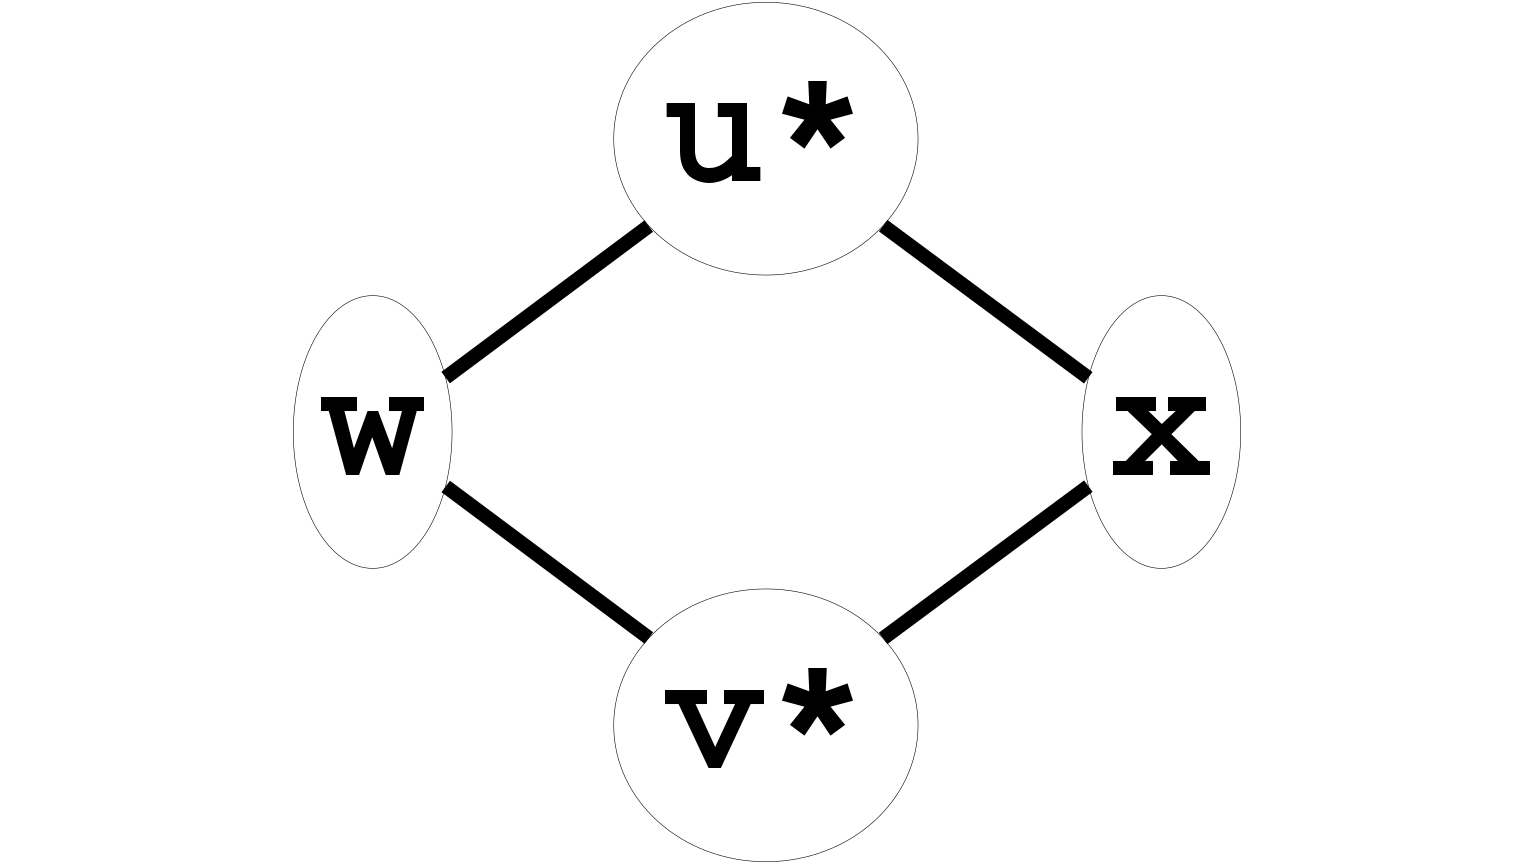
\includegraphics[width=5cm]{square_graph.png}
\makebox[\textwidth]{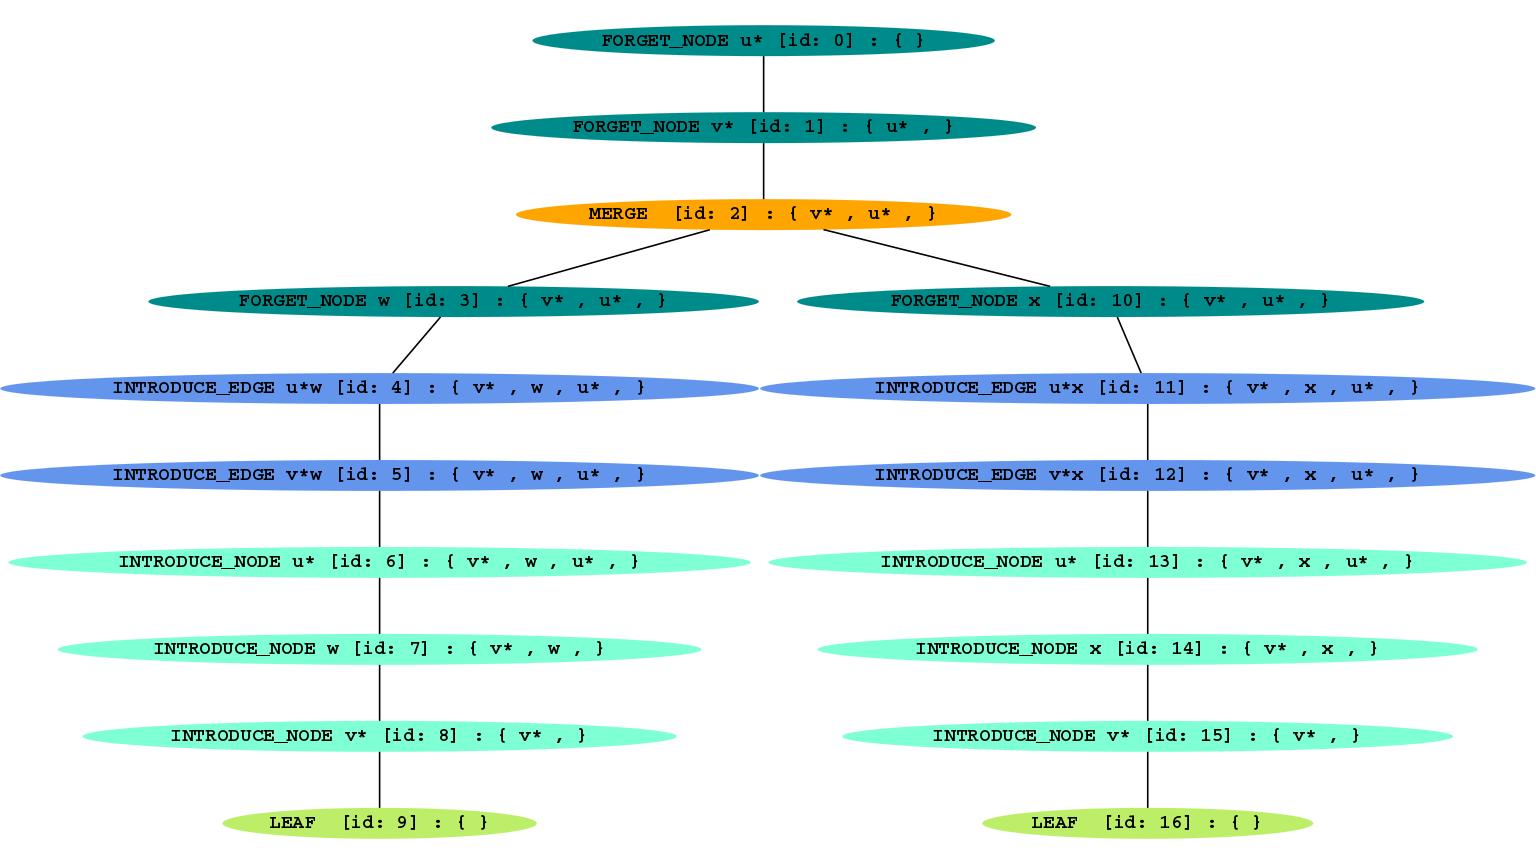
\includegraphics[width=17cm, height=11cm]{square_decomp.png}}
\end{center}


\newpage
	\begin{thebibliography}{9}
		\bibitem{kloks} 
			T. Kloks. 
			\textit{Treewidth. Computations and approximations}. 
			Lecture Notes in Computer Science, 842, 1994.
 
		\bibitem{bodlaender} 
			H. L. Bodlaender. 
			\textit{A linear-time algorithm for nding tree-decompositions of small treewidth}. 
			SIAM J. Comput. 25:6 (1996) 1305-1317
			
		\bibitem{robertson&seymour} 
			N. Robertson and P. D. Seymour. 
			\textit{Graph Minors II. Algorithmic aspects of treewidth}. 
			J. Algorithms 7 (1986) 309-322
 
		\bibitem{knuthwebsite} 
			Knuth: Computers and Typesetting,
			\\\texttt{http://www-cs-faculty.stanford.edu/\~{}uno/abcde.html}
	\end{thebibliography} 



\end{document}
